\documentclass[english]{article}
\usepackage[utf8]{inputenc}
\usepackage[T1]{fontenc}
\usepackage{babel}
\usepackage{amsmath}
\usepackage{graphicx}
\usepackage{fancyhdr}
\usepackage{caption}
\usepackage{subcaption}
\usepackage{hyperref}
\usepackage{float}
\usepackage{numberedblock}
\usepackage{algorithm}
\usepackage[noend]{algpseudocode}
\newcommand{\overleaflogo}{
\includegraphics[height=24pt]{neu.png}}
\pagestyle{fancy}
\fancyhf{}
\renewcommand{\headrulewidth}{0pt}
\setlength{\headheight}{40pt} 
\rhead{\textsc{\overleaflogo}}

\usepackage{mathtools}

\DeclarePairedDelimiter\abs{\lvert}{\rvert}%
\DeclarePairedDelimiter\norm{\lVert}{\rVert}%

% Swap the definition of \abs* and \norm*, so that \abs
% and \norm resizes the size of the brackets, and the 
% starred version does not.
\makeatletter
\let\oldabs\abs
\def\abs{\@ifstar{\oldabs}{\oldabs*}}
%
\let\oldnorm\norm
\def\norm{\@ifstar{\oldnorm}{\oldnorm*}}
\makeatother

\usepackage{listings} %code highlighter
\usepackage{color} %use color
\definecolor{mygreen}{rgb}{0,0.6,0}
\definecolor{mygray}{rgb}{0.5,0.5,0.5}
\definecolor{mymauve}{rgb}{0.58,0,0.82}

\makeatletter
\def\BState{\State\hskip-\ALG@thistlm}
\makeatother
 
%Customize a bit the look
\lstset{ %
backgroundcolor=\color{white}, % choose the background color; you must add \usepackage{color} or \usepackage{xcolor}
basicstyle=\footnotesize, % the size of the fonts that are used for the code
breakatwhitespace=false, % sets if automatic breaks should only happen at whitespace
breaklines=true, % sets automatic line breaking
captionpos=b, % sets the caption-position to bottom
commentstyle=\color{mygreen}, % comment style
deletekeywords={...}, % if you want to delete keywords from the given language
escapeinside={\%*}{*)}, % if you want to add LaTeX within your code
extendedchars=true, % lets you use non-ASCII characters; for 8-bits encodings only, does not work with UTF-8
frame=single, % adds a frame around the code
keepspaces=true, % keeps spaces in text, useful for keeping indentation of code (possibly needs columns=flexible)
keywordstyle=\color{blue}, % keyword style
% language=Octave, % the language of the code
morekeywords={*,...}, % if you want to add more keywords to the set
numbers=left, % where to put the line-numbers; possible values are (none, left, right)
numbersep=5pt, % how far the line-numbers are from the code
numberstyle=\tiny\color{mygray}, % the style that is used for the line-numbers
rulecolor=\color{black}, % if not set, the frame-color may be changed on line-breaks within not-black text (e.g. comments (green here))
showspaces=false, % show spaces everywhere adding particular underscores; it overrides 'showstringspaces'
showstringspaces=false, % underline spaces within strings only
showtabs=false, % show tabs within strings adding particular underscores
stepnumber=1, % the step between two line-numbers. If it's 1, each line will be numbered
stringstyle=\color{mymauve}, % string literal style
tabsize=2, % sets default tabsize to 2 spaces
title=\lstname % show the filename of files included with \lstinputlisting; also try caption instead of title
}
%END of listing package%

\begin{document}

\title{2048 Solver}

\author{Samanjate Sood}

\maketitle
\thispagestyle{fancy}

\begin{abstract}
The popular strategy game 2048 which went viral in 2013-14, though easy to play, can sometimes be tricky at a certain points in the game. I have made use of the expectimax and minimax algorithms, with some scoring heuristic, with an aim to perform better than humans at solving this game.
\end{abstract}

\section*{Background \& Summary}

The 2048\textsuperscript{1} is a single-player video game developed by
by Italian programmer Gabriele Cirulli\textsuperscript{2}. The game is played on a 4x4 board where each cell of the grid can hold a tile. The value of the tile is in powers of two. Initially the board starts with two cells randomly filled with either a tile with a value of 2 or 4. The player can then move in four directions: up, down, left, and right; that is if the move is possible. This then moves all the tiles of the grid in the selected direction, and if two neighbouring tiles are of the same value, they merge to form a tile with a value equal to the sum of the two merged tiles. After each move, a tile randomly spawns in an empty cell whose value is either 2 or 4. This continues till the grid is full and the game ends. The goal of the game is to, as the name suggests, form the 2048 tile; in which case the user wins. It is possible to continue playing and form tiles of higher values, i.e. the mighty 4096 tile. This however becomes tedious and difficult to achieve since it takes a lot time and concentration. My goal for this project is to build an AI that performs better than humans. This is done by looking ahead from one grid state and maximize the grid value of the future by using an evaluation function. All this is done at a relatively faster rate than a human reaction to a game state.

\section*{Question}

As mentioned above, I had set out to build an AI that performs better than humans. Having played the game quite a few times, on an average I was able to achieve the 2048 tile two out of ten times. Having read a few posts on Quora and Reddit, the average human score on this game by humans is not as impressive as that of an AI algorithm. An article on Business Insider\textsuperscript{3} corroborates this claim. After being introduced to different state-search algorithms in my Foundations of Artificial Intelligence class inspired me to write an AI to at least perform better than I. This coupled with a few heuristic functions to evaluate the grid states helped me build this project. An average human would take a few seconds to react to a grid state and then decide upon a move. This AI solves the problem at least 10 times as fast as a human, which in itself is quite impressive.
\section*{Methods}

There are several AI methods that are applicable to this problem. But I decided to formulate this as a state-search problem and then apply two algorithms while comparing the performance of the two. The two algorithms used are Minimax\textsuperscript{4} and Expectimax\textsuperscript{5}. In my implementation, both algorithms work reasonably fast at a depth of 6.

\subsection*{Game Tree}
Even though the game is a single-player game, it can be formulated as a two-players game. There is a player who makes the move, and then there is another player who spawns the 2 or 4 tiles in the empty cells. Thus the game tree would look something as follows:
\begin{figure}[H]
  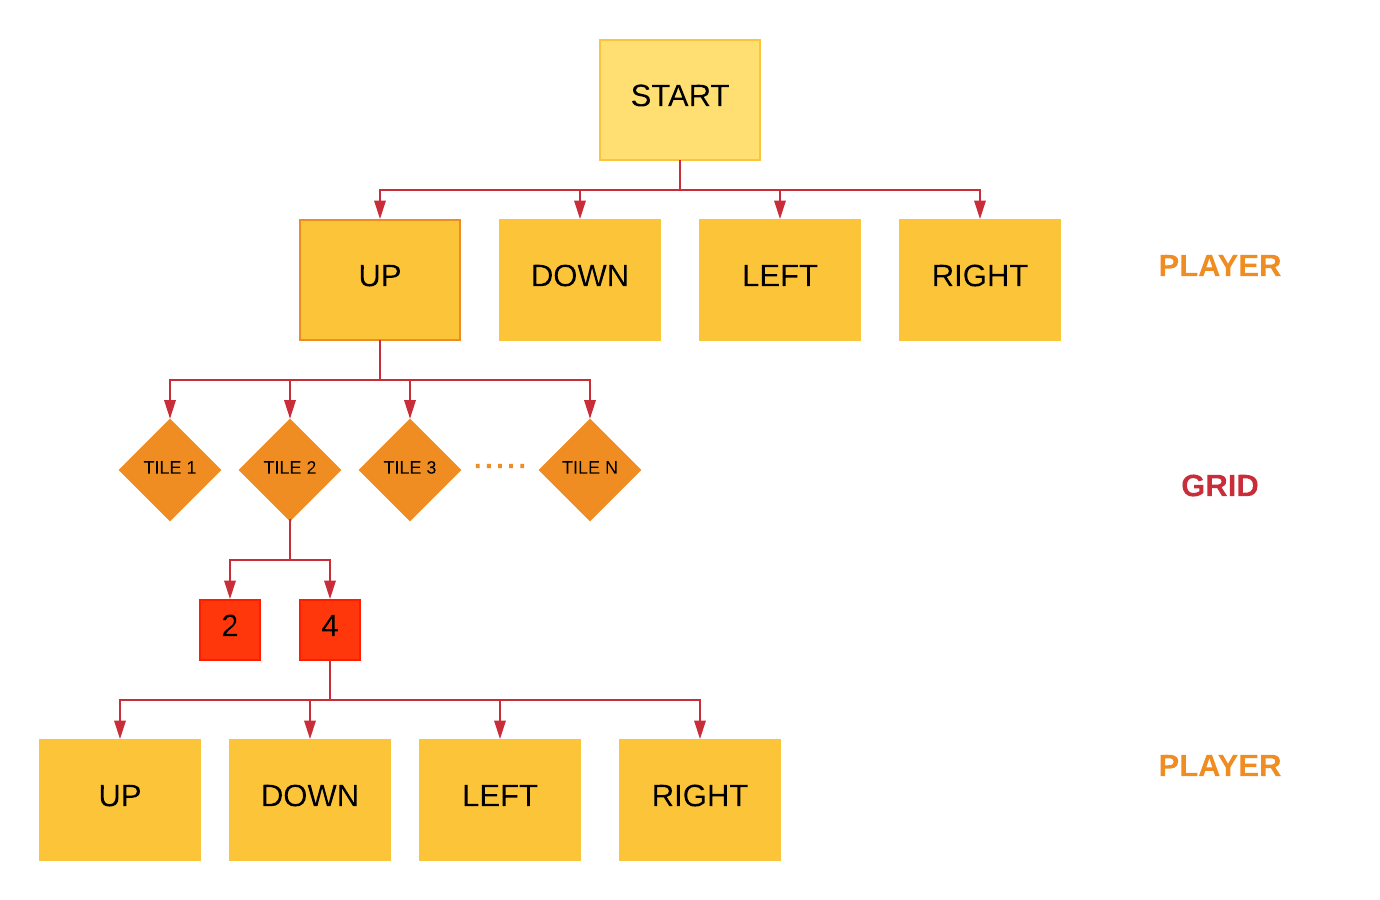
\includegraphics[height=250pt]{Tree.png}
\end{figure}

\subsection*{Minimax}
There are two different options to choose from, for this algorithm. One is that the minimizing player can either return the minimum or the maximum value of the child nodes to their parent node. If you choose to return the minimum value, you would be taking a pessimistic approach and try to follow a path which would lead you to the least worst state. On the other hand, if you return the maximum value, it would be a more optimistic approach and you will follow a path which would potentially lead you to higher state values. Thus, the two players are co-operative and not competitive, as per the traditional minimax algorithm. In either case, it ignores any weight of the other tile spawns. I have implemented the latter approach for this project. The recursive equation and the pseudo-code for the algorithm is as follows:
\begin{displaymath}
\resizebox{.9\hsize}{!}{$minimax(grid, depth, agent) =\begin{cases}
    eval(grid), & \text{depth = 0}.\\
    \max_{dir \in moves(grid)} minimax(move(grid, dir), depth-1, GRID), & \text{agent = PLAYER}.\\
    \max_{cell \in emptyCell(grid)} P(tile) * minimax(insertTile(grid, cell), depth-1, PLAYER), & \text{agent = GRID \& tile $\in$ \{2,4\}}.\end{cases}$}
\end{displaymath}

\begin{algorithm}
\caption{Implementation of the minimax algorithm for a 2048 game}
\begin{algorithmic}[1]
\Procedure{minimax}{grid, depth, agent}
\If {$\textit{depth} = \textit{0}$} \Return $\textit{eval}(grid)$
\ElsIf {$\textit{agent} = \textit{PLAYER}$} 
\State $score \gets 0.0$.
\ForAll {$\textit{dir in } \textit{movesAvailable(grid)}$} 
\State $grid_c \gets clone(grid)$.
\State $move(grid_c, dir)$.
\State $score \gets max(score, minimax(grid_c, depth-1, GRID))$.
\EndFor
\Return $\textit{score}$
\ElsIf {$\textit{agent} = \textit{GRID}$} 
\State $score \gets 0.0$.
\ForAll {$\textit{cell in } \textit{emptyCells(grid)}$} 
\State $grid_2 \gets clone(grid)$.
\State $insertTile(grid_2, cell, 2)$.
\State $score_2 \gets minimax(grid_2, depth-1, PLAYER)$.
\State $grid_4 \gets clone(grid)$.
\State $insertTile(grid_4, cell, 4)$.
\State $score_4 \gets minimax(grid_4, depth-1, PLAYER)$.
\State $score \gets max(score_2, score_4)$.
\EndFor
\Return $\textit{score}$
\EndIf
\EndProcedure
\end{algorithmic}
\end{algorithm}

\subsection*{Expectimax}
This algorithm is not very different from the minimax algorithm. The main difference here is that instead of taking the maximum of the child nodes, we take the weighted average of them. We already know from the source code of the game that probability of the tile 2 spawning is 90\% and the other is 10\%. We can use this information to weigh the two scores of the states where the 2 and the 4 tile spawned. This algorithm takes into account value for each state. The recursive equation and the pseudo-code for the algorithm is as follows:
\begin{displaymath}
\resizebox{.9\hsize}{!}{$expectimax(grid, depth, agent) =\begin{cases}
    eval(grid), & \text{depth = 0}.\\
    \max_{dir \in moves(grid)} expectimax(move(grid, dir), depth-1, GRID), & \text{agent = PLAYER}.\\
    \sum_{cell \in emptyCell(grid)} P(tile) * expectimax(insertTile(grid, cell), depth-1, PLAYER), & \text{agent = GRID \& tile $\in$ \{2,4\}}.\end{cases}$}
\end{displaymath}

\begin{algorithm}
\caption{Implementation of the expectimax algorithm for a 2048 game}
\begin{algorithmic}[1]
\Procedure{expectimax}{grid, depth, agent}
\If {$\textit{depth} = \textit{0}$} \Return $\textit{eval}(grid)$
\ElsIf {$\textit{agent} = \textit{PLAYER}$} 
\State $score \gets 0.0$.
\ForAll {$\textit{dir in } \textit{movesAvailable(grid)}$} 
\State $grid_c \gets clone(grid)$.
\State $move(grid_c, dir)$.
\State $score \gets max(score, expectimax(grid_c, depth-1, GRID))$.
\EndFor
\Return $\textit{score}$
\ElsIf {$\textit{agent} = \textit{GRID}$} 
\State $score \gets 0.0$.
\ForAll {$\textit{cell in } \textit{emptyCells(grid)}$} 
\State $grid_2 \gets clone(grid)$.
\State $insertTile(grid_2, cell, 2)$.
\State $score_2 \gets expectimax(grid_2, depth-1, PLAYER)$.
\State $grid_4 \gets clone(grid)$.
\State $insertTile(grid_4, cell, 4)$.
\State $score_4 \gets expectimax(grid_4, depth-1, PLAYER)$.
\State $score \gets 0.9 * score_2 + 0.1 * score_4$.
\EndFor
\Return $\textit{score}$
\EndIf
\EndProcedure
\end{algorithmic}
\end{algorithm}

\subsection*{Pruning and Optimization}
 In either case Alpha-Beta pruning is not applicable. Since, I am using a co-operative version of the Minimax algorithm, we cannot prune any branches as any value can topple the previously set maximum value. Expectimax algorithms cannot be optimized using pruning anyway. However there are a few optimization steps done while implementing the algorithm. For each states, moves in some directions are impossible. Hence, such branches are never explored and the search-states are reduced. With this optimization, at depth 6, the algorithm works at 1 move per sec in the worst case, and up to 5 moves per sec, depending on the number of empty cells in the current grid state. 

\subsection*{Code}

The implementation of the two algorithms, using JavaScript, are available on my GitHub Repository\textsuperscript{6} and the visual representation on how the algorithms work at depth 6 are on the website\textsuperscript{7} linked below.

\section*{Evaluation and Heuristics}

By far, the hardest part of the building an AI for the game, is creating an efficient heuristic function and comparing two state; What makes one state better than the other? When the two algorithms halts at the depth bound, we need to evaluate the leaf nodes and return a value of the state. The value represents how good that state is and hence the AI can decide whether to pursue that state or not.

The score of the game is not used to evaluate the state at all, since it is biased towards merging tiles. After much experimentation, I found that the best way to evaluate a game state is using a weighted matrix. This matrix has higher weights for cells closer to one chosen corner. These weights are derived from how a human would approach the problem. Only that in this case, we will be able to look six steps ahead and choose the best move way faster than an average human.

\begin{figure}[H]
 \centering
  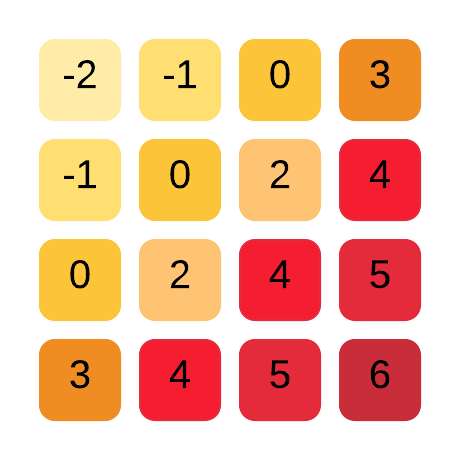
\includegraphics[height=100pt]{matrix.png}
\end{figure}

A higher values of weights at one corner restricts the new tiles to be spawned at the upper left corners. This allows the AI to keep the maximum game activity at the bottom right corner, which helps with merging similar tiles. To ensure that the higher values tiles are collected in one corner, we need to reward the AI with higher score at that corner. We can easily do this incorporating the tile value in our scoring function. This will allow the highest tile to be at the corner and the second biggest tile besides it and so on. Our scoring function would then look like:
\newline
\begin{displaymath}
score = \sum_{c \in Cells_{g}} Weight_{c} * {Tile_{c}}^2
\end{displaymath}

We can further reward the AI for having empty cells in the grid. This can be done by simply multiplying the number of empty cells with its weight. After some experimentation.
\begin{displaymath}
score = score + Weight_e * Cells_{empty}
\end{displaymath}

I was able to find the best performance with $Weight_e = 32.0$.
\newline

This works well, but we still need to make sure that similar valued tiles are side-by-side throughout the grid cells; for them to be merged. This can be done by penalizing for states having isolated tiles. This is done by using the following formula:
\newline
\begin{displaymath}
penalty = \sum_{t \in Tile_g}\sum_{n \in Nbr_{t}} \abs{t_i - n_i}
\end{displaymath}
The final grid value is then calculated using a simple formula:
\begin{displaymath}
value = score - penalty
\end{displaymath}

\section*{Experimentation}

To arrive at the aforementioned solution, there was a lot of experimentation involved. Inspired by other people's work, I started developing an AI that would emulate theirs. At the end of, I was able to add my own spin to their ideas, and came up with a reasonably good AI, that out performs humans.

\subsection*{Related Work}
There are a couple of AI projects that inspired me to build an AI for the game. There is one AI\textsuperscript{8} using the same algorithms that is able reach the 32768 tile 36\% times! It uses the expectimax algorithm but their heuristics are different. This implementation represents the game as a 64-bit unsigned integer, which allows over 100,000 look ups per second! Further, the algorithm is optimized by storing the scores in look-up tables. This by far, would be the start-of-art AI out there, that can solve the 2048 game.
Another one\textsuperscript{9} that I would like to mention is where the implementation is done as an iterative depth search. This is bounded by time, rather than depth. It decides the best move within 100ms and  instead of the second player being the grid, the algorithm "beta prunes" a number of states. This was the starting point of my project, where I was able to incorporate the previously build UI and helper functions like cloning the grid into my project.

\subsection*{Getting There}
Since the start, I have used the minimax and expectimax algorithms to solve the game. That has been a constant throughout and has little to do with experimentation. Hence, I am not going to talk about the two algorithms in this section. The interesting part of the project would be designing the heuristics and measuring their performance. 

The way to tell whether an AI is good or not is fairly simple. If it is able to reach the 2048 tile within reasonable decision time and at high frequencies, then that would be considered to be a good AI. I had first developed an AI where I used the same ideas of monotonicity and smoothness as in the two aforementioned AI's. I was using the functions already in their code. Monotonicity would mean having either strictly increasing or decreasing along the top/down and left/right directions. Smoothness would be the the difference in the values of tile and its neighbours. Furthermore, there is also a rewards for a "merge-ability" from one state to another, which means making sure that same-valued tiles are together. 

Using these measures, I was evaluating all intermediate nodes along a path in the state-space. This was not particularly an efficient solution, since evaluating each state took a lot of time, and I had to compromise with the depth. Hence, I was only able to search at a depth of 4. The performance of the AI wasn't satisfactory either. It was only able to reach 1024 tile at most, with one  lucky run where it achieved the 2048 tile.

Building on this solution, I got rid of the "merge-ability" factor and modified the monotonicity formula a bit. While there was an incremental improvement in performance, it still wasn't still at a satisfactory level.

After this attempt, I got rid of the smoothness function, since the original implementation had a very low weight assigned to it. I had also, completely resigned the monotonicity function, where the new formula would use the weights assigned to a grid cell, multiplying it with the tile value in that cell of the current grid state. At this point, the algorithms and heuristics weren't derived from previous implementations and I was working with completely new code inspired by the business insider article\textsuperscript{3}. This significantly bumped the performance, as I was able to see the 1024 tile more often than not.

At this point, since the depth search was impacting the performance, I stopped evaluating the intermediate states and only considered the leaf nodes to contribute to the final grid value. I was able to perform a state search at depth 6 in a reasonable decision time. This helped me reach the 2048 tile.

I was then only evaluating leaf nodes, with my heuristics helping me to restrict the activity in one corner. There was an award for empty cells. The search was bounded by a depth of 6. The performance was satisfactory, but I wasn't able to reach the 4096 in any of the runs. The 2048 tile was being achieved at about 50\% of the times. I then changed my heuristic to add more stress on higher tiles at the corned by multiplying the weight by the square of the tile value. I also penalized the state for having tiles with more difference adjacent to each other. The result of this change was significant and I was able to get the 2048 tile about 80\% of the times. I have also seen the 4096 tile.

\subsection*{Road Ahead}
While the implementation of the algorithm performs quite well, it still isn't optimal. Designing a heuristics which would achieve the 2048 tile every time, would be the most important part of it. There are other optimizations that can be done, in form of representing the game in a compact way and store scores in look-up tables for faster computation. This would help us search deeper in the state-space and produce optimal results. There is also potential to collect data for each run of the algorithm and decide the weights for each algorithm run. We can then fit a regression model to the data set to decide the weights of the two algorithms.

\section*{Performance}

Based on 50 runs per algorithm, the best run was by the minimax algorithm. It reached the 4096 tile with another 2048 tile besides it before the game stopped. However, the expectimax algorithms performs better across the 50 runs. Figure 1, shows examples for each algorithm's result.
\begin{figure}[H]
\centering
\begin{subfigure}{.5\textwidth}
  \centering
  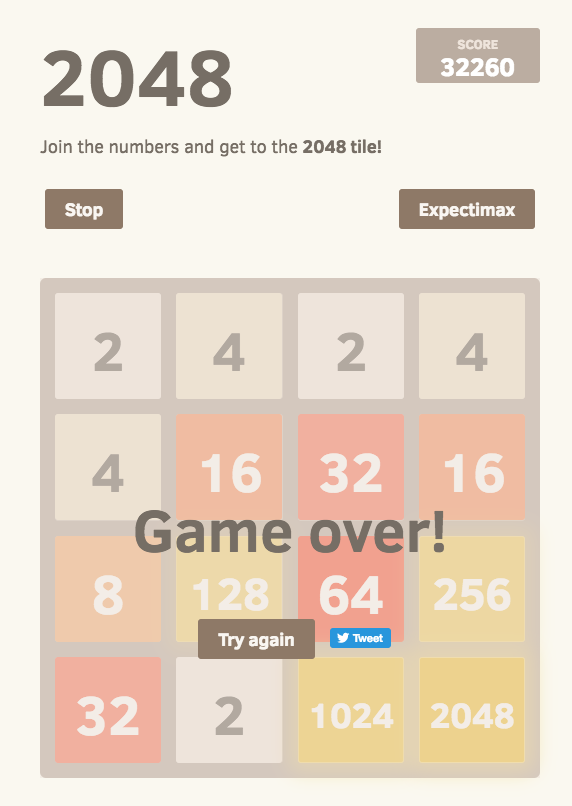
\includegraphics[width=.7\linewidth]{2048.png}
  \caption{Minimax}
  \label{fig:sub1}
\end{subfigure}%
\begin{subfigure}{.5\textwidth}
  \centering
  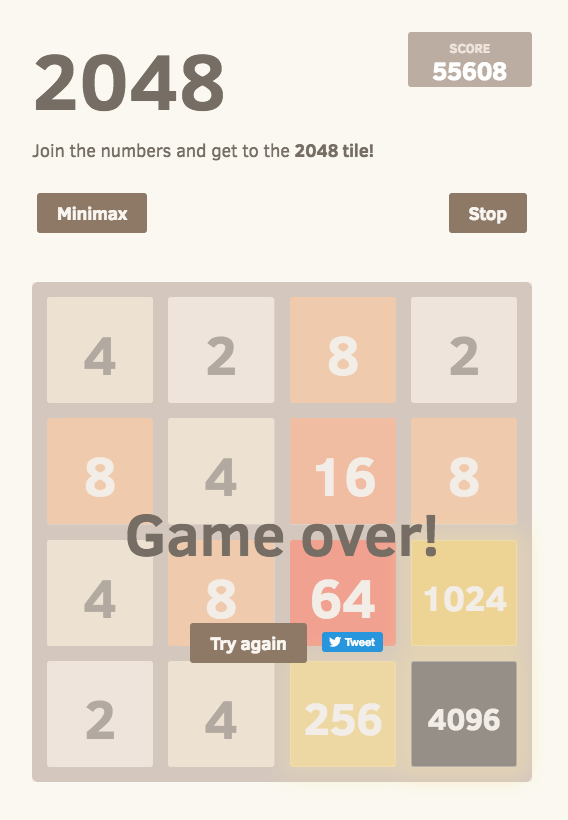
\includegraphics[width=.7\linewidth]{4096.png}
  \caption{Expectimax}
  \label{fig:sub2}
\end{subfigure}
\caption{Examples of two results using the two algorithms.}
\label{fig:test}
\end{figure}

\begin{table}[h!]
\centering
 \begin{tabular}{||c c||} 
 \hline
 Tile & Achieved \\ [2.0ex] 
 \hline\hline
 4096 & 2\% \\
 2048 & 72\% \\
 1024 & 92\% \\
 512 & 100\% \\ [1ex]
 \hline
 \end{tabular}
 \caption{Performance of minimax}
\end{table}

\begin{table}[h!]
\centering
 \begin{tabular}{||c c||} 
 \hline
 Tile & Achieved \\ [2.0ex] 
 \hline\hline
 4096 & 4\% \\
 2048 & 80\% \\
 1024 & 96\% \\
 512 & 100\% \\ [1ex]
 \hline
 \end{tabular}
 \caption{Performance of expectimax}
\end{table}

\section*{References}
1. \href{https://github.com/ovolve/2048-AI}{ovolve} - Used code for UI and helper functions.\newline
2. \href{http://www.businessinsider.com/artificial-intelligence-crushed-all-human-records-in-the-addictive-tile-game-2048--heres-how-2015-5}{BI Article} - Heuristics design based on this idea. 

\section*{Bibliography}
1. \href{https://gabrielecirulli.github.io/2048/}{2048} - The original game. \newline
2. \href{https://github.com/gabrielecirulli}{GitHub Account}. - Gabriele Cirulli \newline
3. \href{http://www.businessinsider.com/artificial-intelligence-crushed-all-human-records-in-the-addictive-tile-game-2048--heres-how-2015-5}{Artificial Intelligence crushed all human records in the addictive tile game 2048 — here's how} - Business Insider Article by Randy Olson. \newline
4. \href{https://en.wikipedia.org/wiki/Minimax}{Minimax Algorithm}. \newline
5. \href{https://en.wikipedia.org/wiki/Expectiminimax_tree}{Expectimax Algorithm}. \newline
6. \href{https://github.com/samanjate/2048-solver}{My Implementation of the algorithm using JavaScript}. \newline
7. \href{https://twenty48-solver.herokuapp.com/index.html}{Visual Representation of the two algorithms}. \newline
8. \href{https://stackoverflow.com/questions/22342854/what-is-the-optimal-algorithm-for-the-game-2048}{What is the optimal algorithm for the game 2048?}. - A stack-overflow article with discussion on the best AI to solve the game. \newline

\end{document}